\section{Enfoque técnico}

\begin{figure*}[t]
    \centering
    \vspace{-3mm}
    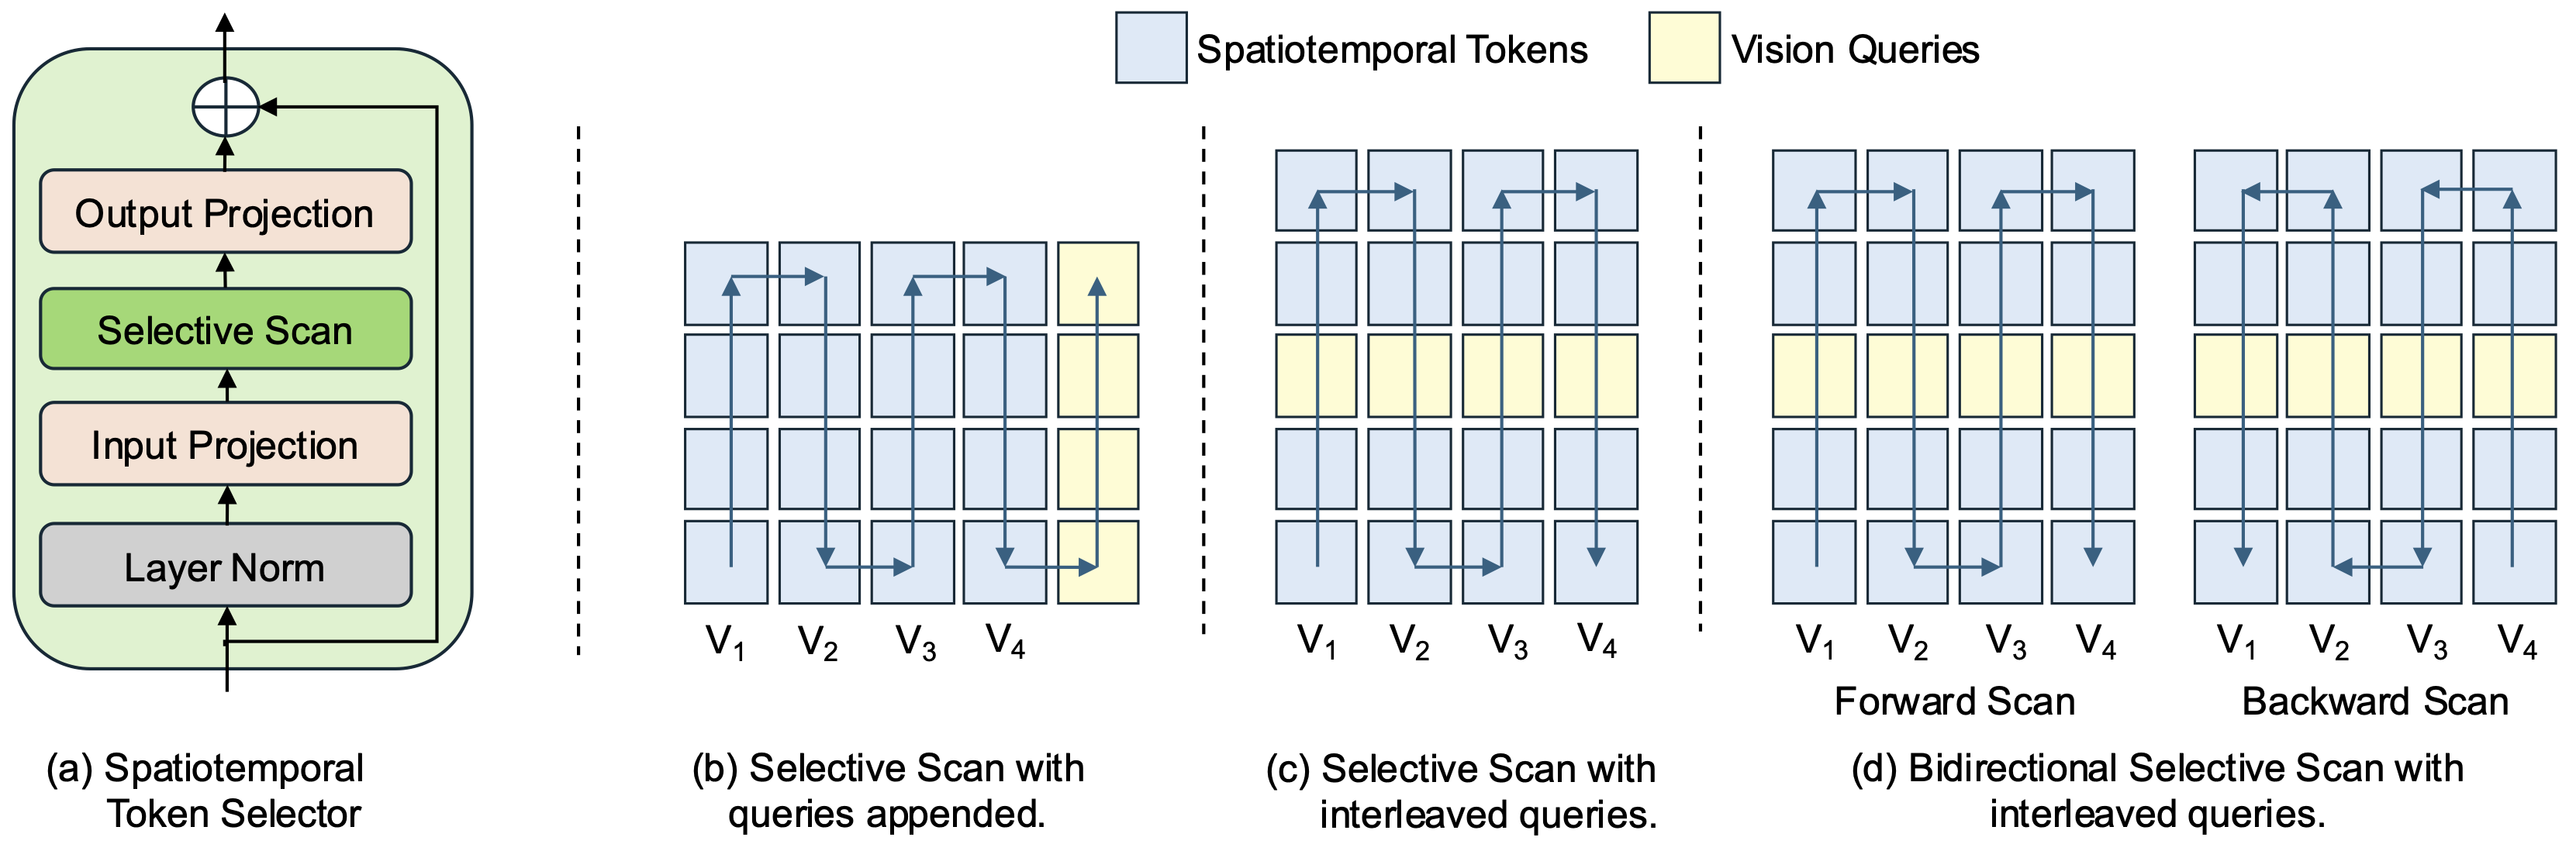
\includegraphics[width=\textwidth]{figures/scan.png}
    \vspace{-8mm}
    \caption{\small{(a): Arquitectura de nuestro Spatiotemporal Token Selector. (b): El selective scan tradicional, con queries añadidas al inicio o al final de la secuencia, introduce sesgos posicionales que a menudo conducen a un rendimiento subóptimo. (c) Proponemos intercalar las queries de manera uniforme para capturar más equitativamente las interacciones entre tokens espaciotemporales a lo largo del video. (d) Además, introducimos una operación bidirectional selective scan (forward y backward) para mejorar aún más el modelado de largo alcance.}}
    \vspace{-5mm}
\label{fig:scan}
\end{figure*}

Presentamos \model, un multimodal large language model (MLLM) diseñado para long-range video question answering. \Cref{fig:model} ilustra la arquitectura general. Nuestro modelo consta de un image encoder estándar~\cite{dosovitskiy2020image}, un spatiotemporal token selector y un LLM decoder~\cite{llama3.2}. Primero, codificamos cada input video frame de manera independiente usando el image encoder y extraemos características a nivel de patch (tokens) de cada frame. Luego, utilizamos un spatiotemporal token selector, que reduce la secuencia de tokens espaciotemporales de entrada en más de un orden de magnitud (por ejemplo, 16$\times$) para permitir un procesamiento eficiente por parte del LLM posterior. En concreto, utilizamos el selective-scan structured state-space model~\cite{gu2023mamba} para diseñar nuestro token selector. Nuestro spatiotemporal token selector modela eficientemente las dependencias espaciotemporales de largo alcance en el video de entrada y selecciona solo los tokens más relevantes del amplio conjunto de entrada. Finalmente, la secuencia comprimida de tokens se pasa al LLM junto con la pregunta en lenguaje natural para generar la respuesta. En las siguientes subsecciones, ofrecemos una discusión detallada de cada componente de nuestro modelo.

\subsection{Image Encoder} 
\label{sec:image selector}

Usamos un vision transformer estándar~\cite{dosovitskiy2020image} para codificar cada video frame de manera independiente. Sea $V = (V_1, ...,V_t, ..., V_T) \in\mathbb{R}^{T\times 3\times H\times W}$ el input video compuesto por $T$ frames $V_t\in\mathbb{R}^{3\times H\times W}$, donde los $3$ canales codifican color en formato RGB, $H$ es la altura y $W$ es el ancho de cada frame. Primero, dividimos cada frame en patches no superpuestos de tamaño ($p\times p$). Luego, se aplica un image encoder $f_I$ para extraer características espaciales (tokens) $z_t\in\mathbb{R}^{h \times w \times d}$ de cada frame $V_t$:
\begin{equation}
    \begin{aligned}
    z_t &= f_I(V_t).
    \end{aligned}
\end{equation} 
donde $h=H/p$, $w=W/p$ y $d$ es la dimensión de las características.
Después, las características de cada frame se concatenan para producir la secuencia de tokens espaciotemporales $\mathbf{Z}\in\mathbb{R}^{T \times h \times w \times d}$. Denotamos el número total de tokens por $L=T\times h \times w$.


\subsection{Spatiotemporal Token Selector}
\label{sec:token selector}

El spatiotemporal token selector tiene dos objetivos principales: (1) capturar dependencias de largo alcance a partir de la secuencia de tokens espacio-tiempo producida por el image encoder y (2) seleccionar los tokens más relevantes dentro de la información altamente redundante típica de los videos largos. Esta tarea es desafiante debido a la gran cantidad de tokens espacio-tiempo generados por el image encoder a lo largo del video. Usar self-attention convencional sería computacionalmente prohibitivo debido a su costo cuadrático respecto de la longitud de la secuencia. Para abordar este problema, usamos un token selector basado en selective scan~\cite{gu2023mamba}, que (1) modela eficientemente dependencias temporales de largo alcance con costo computacional lineal y (2) filtra tokens redundantes, reteniendo solo los más relevantes de la larga secuencia de entrada.


\Cref{fig:scan}(a) ilustra nuestro spatiotemporal token selector. Primero, inicializamos una secuencia de visual queries $\mathbf{Q}\in\mathbb{R}^{T' \times h' \times w' \times d}$ usando una capa adaptive 3D average pooling aplicada sobre los tokens espaciotemporales $\mathbf{Z}$. Aquí, $N=T' \times h' \times w'$ es el número de queries, que es significativamente menor que el número de tokens espaciotemporales de entrada $L=T\times h \times w$, es decir, $N<<L$. En nuestra implementación, la entrada consta de $64 \times 40 \times 40=102,400$ tokens, mientras que el número de queries es $16 \times 20 \times 20=6,400$. Así, el selector aplica una razón de compresión de $16\times$.

Aunque la operación de pooling proporciona una buena inicialización para las visual queries, no captura dependencias espaciotemporales de largo alcance ni detalles de grano fino del input video. Para cerrar esta brecha, aplicamos un mecanismo selective-scan. Primero, concatenamos las visual queries con los tokens espaciotemporales $Z$, produciendo una secuencia combinada de tokens $\mathbf{Z'} \in \mathbb{R}^{L' \times d}$, donde $L' = L + N$. Luego aplicamos layer normalization a $\mathbf{Z'}$, seguida de una capa selective-scan para capturar dependencias de largo alcance e información crítica de grano fino a partir de los tokens espaciotemporales de entrada. Se añade una residual connection después de la capa selective-scan. Finalmente, las $N$ output queries $\mathbf{Q'}$ se extraen de la secuencia combinada $\mathbf{Z'}$ y se pasan al LLM. Estas operaciones se expresan mediante las siguientes ecuaciones:
\begin{equation}
    \begin{aligned}
    &\mathbf{Z'} = [\mathbf{Z}; \mathbf{Q}], \\
    &\mathbf{Z}_{res} = \mathbf{Z'} \\
    &\mathbf{Z'} = \text{Selective-Scan}(\text{LN}(\mathbf{Z'})) \\
    &\mathbf{Z'} = \mathbf{Z}_{res} + \mathbf{Z'}\\
    &\mathbf{Q'} = \text{Extract}(\mathbf{Z'})
    \end{aligned}
\end{equation}

Además, nuestro módulo token selector incorpora adaptaciones de diseño simples pero efectivas para hacerlo adecuado para procesar entradas de video largas, como se ilustra en la Figura~\ref{fig:scan}(c,d) y se describe a continuación.

\subsubsection{Interleaved Queries} Una forma directa de concatenar queries con los tokens espacio-tiempo es anexar las queries al final, como se muestra en \Cref{fig:scan}(b). Sin embargo, este enfoque puede introducir sesgos, ya que sitúa las queries más cerca de los tokens de la parte final del video, lo que potencialmente limita la interacción con frames tempranos y, por lo tanto, pierde contexto del comienzo del video. Para resolver esto, intercalamos las queries entre los tokens espaciotemporales a intervalos regulares, como se muestra en \Cref{fig:scan}(c). Al distribuir uniformemente las queries a lo largo de la secuencia, nuestro diseño permite interacción con tokens de todas las partes del video, favoreciendo una representación más equilibrada y completa.

\subsubsection{Bidirectional Scan} El selective scan original, desarrollado para secuencias 1D, es subóptimo para tareas de visión porque carece de conciencia espacial. Para abordar esta limitación, aplicamos un bidirectional scan (\Cref{fig:scan}(c))~\cite{li2025videomamba}, que realiza un recorrido forward-and-backward sobre los visual tokens. Este recorrido mejora la capacidad del modelo para capturar estructura espaciotemporal, aumentando su efectividad en tareas de video modeling.

\subsubsection{Question-Conditioned Token Selection} También exploramos una variante del token selector en la que anteponemos los tokens extraídos de la pregunta textual a los tokens espaciotemporales antes de pasarlos al token selector. Esta variante mejora la capacidad del modelo para seleccionar los tokens más relevantes al tener en cuenta el contexto proporcionado por la pregunta. La operación se expresa como:
\begin{equation}
    \begin{aligned}
    &\mathbf{Z'} = [\mathbf{X};\mathbf{Z}; \mathbf{Q}], \\
    \end{aligned}
\end{equation}
donde $\mathbf{X}$ representa la pregunta tokenizada por el LLM. Luego, la secuencia combinada de tokens $\mathbf{Z'}$ se pasa al token selector como se describe en \Cref{sec:token selector}.

\subsection{LLM Decoder}

Usamos un LLM decoder $f_L$ para generar una respuesta textual $R$ a partir de la concatenación de la pregunta de entrada tokenizada $\mathbf{X}$ y el conjunto de visual queries $\mathbf{Q'}$ generadas por el spatiotemporal token selector:
\begin{equation}
    \begin{aligned}
    \mathbf{R} &= f_L(\left[ \mathbf{X}; \mathbf{Q'}\right]).
    \end{aligned}
\end{equation}
